%%%%%%%%%%%%%%%%%%%%%%%%%%%%%%%%%%%%%%%%%%%%%%%%%%%%%%%%%%%%%%%%%%%%%%%%
%                                                                      %
%     File: Thesis_Versat.tex                                      %
%     Tex Master: Thesis.tex                                           %
%                                                                      %
%     Author: Andre C. Marta                                           %
%     Last modified :  2 Jul 2015                                      %
%                                                                      %
%%%%%%%%%%%%%%%%%%%%%%%%%%%%%%%%%%%%%%%%%%%%%%%%%%%%%%%%%%%%%%%%%%%%%%%%

%JTS: replace ' ' with '~' between word and \ref or \cite in the whole document
%not only in this file

\chapter{CGRA Simulation}
\label{chapter:CGRA}

As referred before in this work, CGRA architectures have some big differences
when compared with dedicated circuits. This poses difficulties in some areas,
with one of these areas being the simulation of the developed
architectures. Unlike a dedicated circuit, in a CGRA the reconfigurable
interconnects between the functional units allow to build zillions of different
datapaths at run-time. This is an overhead compared to simulating the various
datapaths separately without simulating the reconfigurable infrastructure.

For FPGAs this problem is even worse as the reconfigurable infrastructure is
fine grain and there are small Look Up Tables (LUTs) instead of high-level FUs
like in CGRAs, and even more programmable interconnects. For this reason the
FPGA fabric is never simulated, only the circuits that are mapped onto it are.

As a result, simulating CGRAs with event-driven simulators will result in
lengthy simulation times. Consequently, finding a valid alternative to simulate
CGRAs (in this particular case, the Versat architecture) could save an important
amount of time and money during the development of applications for this type of
architectures.

Using cycle-accurate simulators could be a good alternative to speed up CGRA
simulations. As seen in the previous chapter, the use of a cycle-accurate
simulator like Verilator could cut considerably the simulation time, reducing
it, at least, by a factor of 2 (see Fig~\ref{fig:performance}). It also has the
advantage of having no additional cost, since Verilator is open source. However,
the CGRA (or any other circuit) should not be tested exclusively with a
cycle-accurate simulator, since their results don't have in account the
propagation delays inside the CGRA, and also make some simplifications regarding
the signals state. This is specially true if the CGRA is in constant development
as is the case for Versat.

Another alternative is doing simulations at a high-level, instead of doing them
at the RTL level. High-level simulation techniques have been applied in
different types of circuits, like processors, with good results. However, for
CGRA there is an additional difficulty compared to regular processors for this
type of simulations because of the reconfiguration process. Two examples of
approaches to high-level simulation are presented next: one that proposes a
cycle-accurate simulator~\cite{chen:CGRA}, and another one that proposes a
framework for high-level simulation of CGRAs~\cite{pasha:CGRA}.


\section{High-level cycle-accurate simulator}
\label{section:hlcycle}

The high-level cycle-accurate approach proposed in~\cite{chen:CGRA} introduces
the concept of a timing-constrained datapath. In CGRAs there is not a well
defined pipeline structure due to the reconfigurable interconnects. The pipeline
is formed on the fly with registers or memories being used to save the
intermediate results between the different datapaths.

With this in mind, a register-centric synthesis technique is used using a
timing-constrained datapath rooted at a chosen register. For the example in
Figure~\ref{fig:datapaths}, the datapath is rooted at the register R0, with the
different paths being tracked down within the timing constraint given. These
datapaths can finish either on a circuit input or on an intermediate register.

\begin{figure}[!htb]
	\centering
	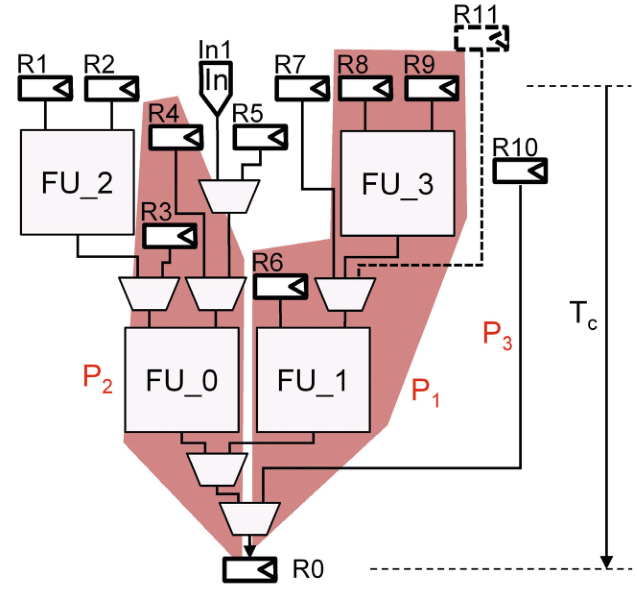
\includegraphics[width=0.6\textwidth]{Figures/Datapaths.png}
	\caption{Timing-constrained datapath example~\cite{chen:CGRA}.}
	\label{fig:datapaths}
\end{figure}

The timing-constrained datapaths will be extracted and used by the compiler,
being converted into a pattern graph of FUs. In this way, the simulation becomes
a signal flow graph simulation, being performed via a routine that updates the
value of all registers and output ports on each clock cycle. For the
register/port udpate routine the obtained graph will be traversed, starting on
the root register, and evaluating all the possible paths. This means that the
simulator only does the necessary operations for the existent configuration
bits, and also that the worst case for the simulation execution time will be
proportional to the number of configuration bits available on the longest path
of the flow graph.

The main simulation routine uses three main components: Input Read,
Register/Port Update (described previously) and State Update. The Input Read is
responsible for reading all the inputs on each clock cycle, and the
Register/Port Update for updating all the values of registers that need to be
updated.

%JTS: what about State Update?

To evaluate the performance of this simulator, multiple simulations were made,
using two different CGRAs: CGRA-1 (modelled similarly to ADRES architecture~\cite{mei:reconfigurable}) and CGRA-2 (similar to~\cite{chen:flexdet}), and
running six different application kernels (3 on each CGRA). Those kernels were
run with different timing constraints, being noted that, while in CGRA-1 the
simulation time increased linearly with the timing constraint, in CGRA-2 the
simulation time did not increase so much. This happened because the CGRA-2 had a
well defined pipeline architecture, along with less complex interconnections.

%JTS: did not get this. Are you sure you understand this?

The simulations speed was compared with some commercially available simulators
(Synopsys VCS-MX 2011.03 and Verilator 3.853), using a system with an AMD Phenom
II X4 955 CPU and 8 GB of memory. To run the simulations the timing constraint
was set to 3 FUs, since the performance of the kernels is the same as without
timing constraint. Both the generated high-level simulator and Verilator were
compiled with GCC 4.4.7. The obtained results are shown in Figure~\ref{fig:hlperformance}, normalized with the simulation time for the high-level
simulator.

\begin{figure}[!htb]
	\centering
	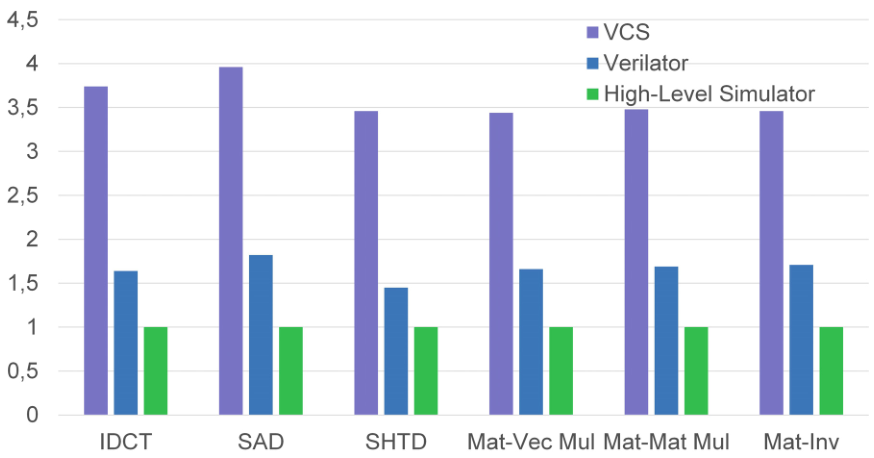
\includegraphics[width=0.8\textwidth]{Figures/hlperformance.png}
	\caption{Performance comparison between the high-level and other commercially available simulators~\cite{chen:CGRA}.}
	\label{fig:hlperformance}
\end{figure}

From the results in Figure~\ref{fig:hlperformance} it can be seen that the
high-level simulator is almost 4 times faster than Synopsys VCS and around 1.5
times faster than Verilator. This was already expected given that, while the
high-level simulator only considers the values in the registers after each
execution cycle, the other simulators also evaluate the intermediate signals.

\section{CGRA high-level simulation framework}
\label{section:framework}

The framework presented in~\cite{pasha:CGRA} provides a high-level simulation
and optimization solution for a given mesh-based CGRA. It accepts applications
written in C, generating the corresponding VHDL description for the target CGRA,
and it can be divided into two main parts: C to netlist transformation and
netlist to CGRA mapping.

The C to netlist transformation relies on GeCoS~\cite{l'hours:FPGA}, an
open-source compiler mainly used for ASIPs (Application Specific Instruction Set
Processors) to compile the C code, generating a data flow graph that represents
the original C code. This was made using GeCoS direct acyclic graphs generation
capabilities. To transform the generated graphs into netlists for the target
CGRA, a parser was created. In the resulting netlist, each ALU corresponds to a
node in the original graph.

For the netlist to CGRA mapping, the previously generated netlists are placed
into the target CGRA, using a simulated annealing algorithm. The placement and
routing algorithms for netlist to CGRA mapping used are independent of the CGRA
architecture, so they can be used for exploring different architectures. In the
end an estimation of the area used is calculated.

The performance of the developed framework was only compared with FPGAs, using
an open-source high-level simulation tool targeted at FPGA generation.
%JTS: what tool? why does the fpga need to be generated ?
However, instead of comparing the CGRA simulation performance with the FPGA
simulation
%JTS: or execution ?
performance, it would be more useful (in the scope of this report) to compare
how this new framework performs simulating a CGRA when compared with other
commercial HDL simulators, using the same architecture.
